\documentclass[a4paper, 11pt]{article}
\usepackage{theme}
\usepackage{shortcuts}
\addbibresource{ref.bib}

\title{Semantic Classification of 3D point clouds with multiscale spherical neighborhoods}
\author[1, 2]{Ines VATI}
\affil[1]{École des Ponts ParisTech, Champs-sur-Marne, France}
\affil[2]{MVA, ENS Paris-Saclay, Cachan, France}
\affil[1, 2]{Email \email{ines.vati@eleves.enpc.fr}}


\date{}

\begin{document}
\maketitle
\begin{abstract}
    
\end{abstract}
\textbf{Keywords.} 3D point clouds, semantic classification, multiscale, spherical neighborhoods, Random Forest Classifier


\section{Introduction}
\section{Proposed method}

\section{Experiments and results}

\subsection{Influence of neighborhood definition}
\subsection{Influence of scales}
\subsection{Additional features and feature importance comparaision}

\subsection{NPM3D dataset}

\subsection{Paris-rue-cassette dataset}

\begin{figure}
    \begin{subfigure}{0.5\textwidth}
        \centering
        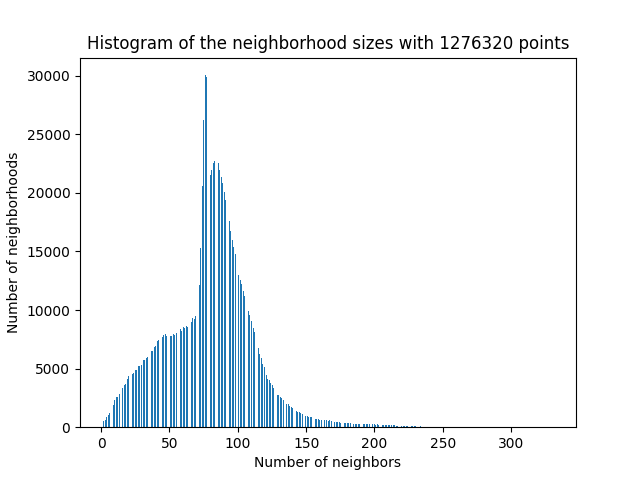
\includegraphics[width=\textwidth]{../Figures/neigh_hist_scale0.png}
        \caption{$s=0$, $r=0.5m$}
    \end{subfigure}
    \hfill
    \begin{subfigure}{0.5\textwidth}
        \centering
        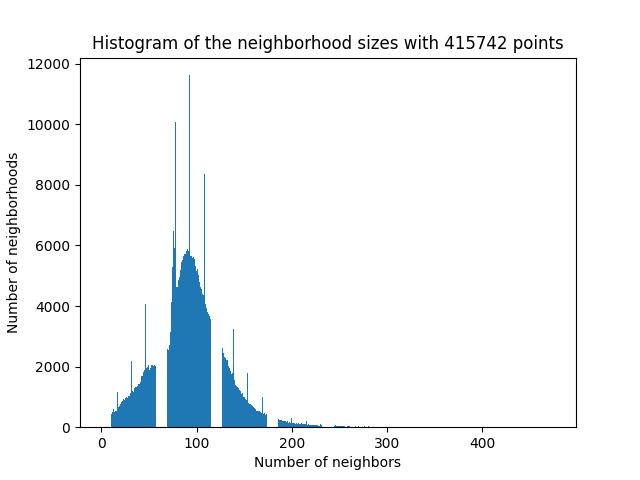
\includegraphics[width=\textwidth]{../Figures/neigh_hist_scale1.png}
        \caption{$s=1$, $r=1m$}
    \end{subfigure}
    \hfill
    \begin{subfigure}{0.5\textwidth}
        \centering
        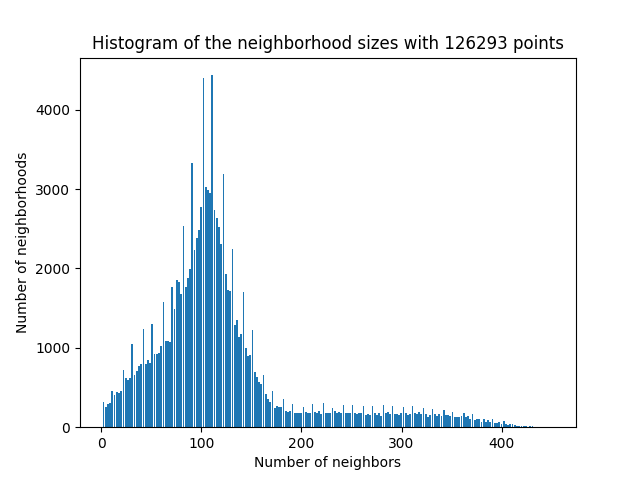
\includegraphics[width=\textwidth]{../Figures/neigh_hist_scale2.png}
        \caption{$s=2$, $r=2m$}
    \end{subfigure}
    \hfill
    \begin{subfigure}{0.5\textwidth}
        \centering
        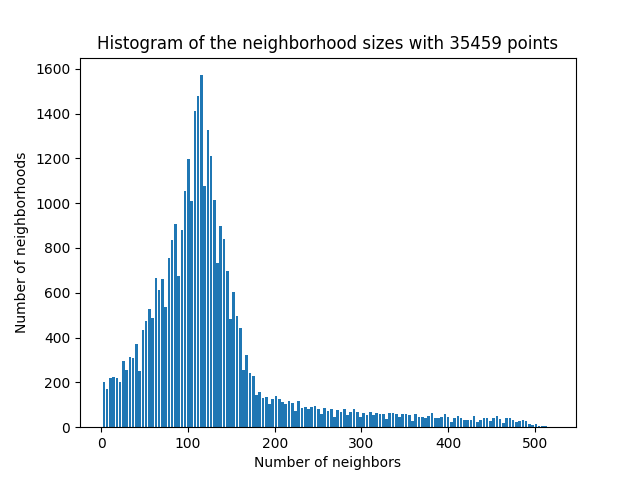
\includegraphics[width=\textwidth]{../Figures/neigh_hist_scale3.png}
        \caption{$s=3$, $r=4m$}
    \end{subfigure}
    \caption{Histogram of the number of points in the neighborhood of each point for different scales $s$ on the subsampled Paris-rue-Cassette Dataset.}
\end{figure}

\section{Improvement proposals}
\subsection{Speed up attempts}
I tried to compute the features on multiple CPU processes using \texttt{multiprocessing} package to speed for loops. Howerver, objects placed on multiprocessing queues are pickled, transferred over the queue, and then unpickled. The pickling and unpickling steps add overhead, and for large objects this overhead can be significant. This is because large objects require more data to be pickled and transferred, and the unpickling step requires reconstructing the entire object. 

Then, I tried Numba which is a just-in-time compiler for Python that works best on code that uses NumPy arrays and functions. Computing the features of 40 points with 4 scales on the subsampled points (about 1,288,215 points) took 54 seconds. I computed and saved the features of all points, excluding the points with label 0. It took in [time ] hours. 

\subsection{Active learning}

\subsection{Classification methods}
Random Forest classifier is usually used for semantic classification of 3D point clouds \cite{thomas_semantic_2018,hackel_fast_nodate}. Indeed, it is directly applicable to multi-class problems and has been shown to yield good results in reasonable time on large point clouds \cite{weinmann_semantic_2015,atik_machine_2021}. I use Gini index as splitting criterion.

However, other classification methods could be considered \cite{atik_machine_2021}. 

Boosting is an ensemble machine learning approach. Boosting algorithms combine multiple low accuracy or weak models to create high accuracy or strong model. Among the most popular boosting algorithms are AdaBoost, Gradient Boosting, and XGBoost.

\section{Conclusion}

In 2019, Thomas et al. \cite{thomas_kpconv_2019} propose a deep learning approach for semantic segmentation using convolutions on point clouds.
\printbibliography

\appendix

\section{Multiscale features computation}
\begin{table}[H]
    \centering
    \begin{tabular}{|c||c|}
    \hline   
    Sum of eigenvalues & $\sum \lambda_i$ \\[1ex]
    \hline
    Omnivariance & $(\prod \lambda_i)^{(1/3)}$\\[1ex]
    \hline
    Eigenentropy & $-\sum \lambda_i \ln(\lambda_i)$\\[1ex]
    \hline
    Linearity & $\frac{\lambda_1 - \lambda_2}{\lambda_1}$\\[1ex]
    \hline
    Planarity & $\frac{\lambda_2 - \lambda_3}{\lambda_1}$\\[1ex]
    \hline
    Sphericity & $\frac{\lambda_3}{\lambda_1}$\\[1ex]
    \hline
    Change of curvature & $\lambda_1 - \lambda_3$\\[1ex]
    \hline
    Verticality ($\times2$) & $|\arcsin(\dotp{e_i}{e_z})|_{i=1, 3}$ \\[1ex]
    \hline
    Absolute moment ($\times6$) & $\frac{1}{|\mathcal{N}|}|\sum_{j\in\mathcal{N}} \dotp{p_j - \mathbf{p}}{e_i}^k|_{k = 1, 2;\; i = 1, 2, 3}$\\[1ex]
    \hline  
    Vertical moment ($\times2$) & $\frac{1}{|\mathcal{N}|}|\sum_{j\in\mathcal{N}} \dotp{p_j - \mathbf{p}}{e_z}^k|_{k=1, 2}$ \\[1ex]
    \hline
    Number of points & $|\mathcal{N}|$\\[1ex]
    \hline
    \end{tabular}
    \caption{Geometric features \cite{thomas_semantic_2018} of point $\mathbf{p}$ whose neighborhood is $\mathcal{N}$.}
    \label{tab:thomas_feat}
\end{table}
\begin{table}[H]
    \centering
    \begin{tabular}{|c||c|}
        \hline
        Vertical range & $z_{max} - z_{min} $\\[1ex]
        Height below & $\mathbf{p}_z - z_{min} $ \\[1ex]
        Height above & $z_{max} - \mathbf{p}_z$\\[1ex]
        \hline
    \end{tabular}
    \caption{Additional height feature from \cite{hackel_fast_nodate} and \cite{mohamed_improvement_2022}, where $z_{max} = \umax{j\in\mathcal{N}}p_{j,z}$ and $z_{min} = \umin{j\in\mathcal{N}} p_{j,z}$}
\end{table}

\end{document}